\documentclass[../DoAn.tex]{subfiles}
\begin{document}

\section{Khảo sát hiện trạng}
\label{section:2.1}

Hiện nay trên thị trường đã có một số ứng dụng hỗ trợ việc tìm và đặt người lái hộ như: FastGo, ViSafe, GOCheap,...
Dưới đây là đánh giá về các ứng dụng này để tìm hiểu về các tính năng cũng như hạn chế của chúng:

\textbf{FastGo}: FastGo là một trong những ứng dụng thuê lái xe hộ khi say được yêu thích hiện nay. 
Được phát triển bởi công ty cổ phần FastGo Việt Nam, app này cung cấp dịch vụ lái xe chuyên nghiệp và an toàn cho người sử dụng.
\begin{itemize}
    \item Ưu điểm:
      \begin{itemize}
        \item Giao diện đơn giản, dễ sử dụng
        \item Bảo mật thông tin cá nhân
        \item Tính năng đặt xe và theo dõi hành trình dễ dàng
        \item Hỗ trợ khách hàng 24/7
      \end{itemize}
    \item Hạn chế:
      \begin{itemize}
        \item Cần phải kết nối mạng ổn định
        \item Không có tính năng đón khách
      \end{itemize}
\end{itemize}

\textbf{ViSafe}: ViSafe là một ứng dụng thuê lái xe hộ khi say được phát triển bởi Công ty Cổ Phần An Toàn Giao Thông Việt Nam. App này nhắm đến việc cung cấp dịch vụ an toàn và chất lượng cho người sử dụng.
\begin{itemize}
    \item Ưu điểm:
      \begin{itemize}
        \item Giao diện đơn giản, dễ sử dụng
        \item Bảo mật thông tin cá nhân
        \item Hỗ trợ khách hàng 24/7
        \item Đa dạng tính năng
      \end{itemize}
    \item Hạn chế:
      \begin{itemize}
        \item Không có tính năng theo dõi hành trình
      \end{itemize}
\end{itemize}

\textbf{GOCheap}: GOCheap là một trong những app đặt lái xe hộ khi say tuyệt vời nhất ở thời điểm hiện tại. Ứng dụng này được phát triển và quản lý bởi Công ty TNHH GOCheap. Ứng dụng này nhắm đến mục tiêu cung cấp dịch vụ thuê lái xe hộ chất lượng và uy tín nhất cho người dùng.
\begin{itemize}
    \item Ưu điểm:
      \begin{itemize}
        \item Tiện lợi, nhanh chóng
        \item Dịch vụ chất lượng
        \item Bảo mật tốt
        \item Hỗ trợ 24/7
      \end{itemize}
    \item Hạn chế:
      \begin{itemize}
        \item Giao diện chưa không thân thiện
      \end{itemize}
\end{itemize}


\section{Tổng quan chức năng}
\label{section:2.2}

\subsection{Biểu đồ use case tổng quát}
\label{subsection:2.2.1}
\begin{figure}[H]
    \centering
    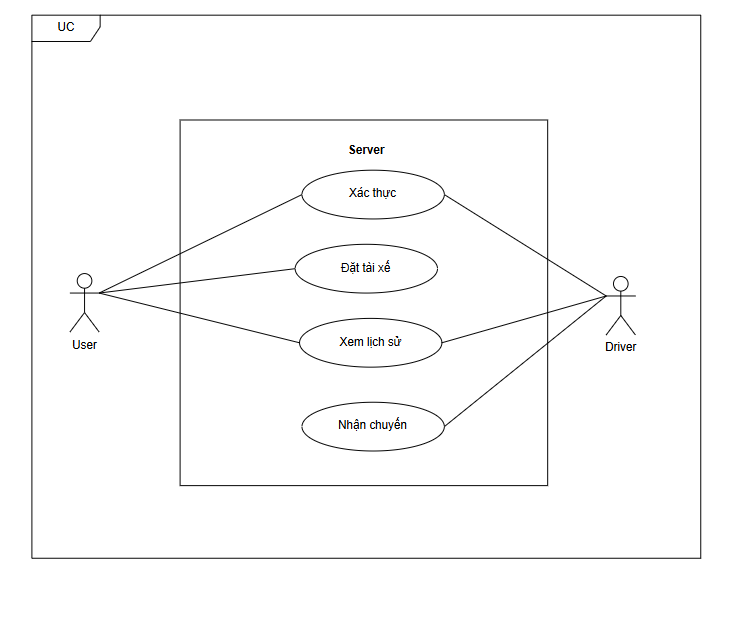
\includegraphics[width=0.8\textwidth]{Hinhve/Usecase_tong_quan.png}
    \caption{Biểu đồ use case tổng quát}
    \label{fig:use_case_total}
\end{figure}
Hệ thống gồm 2 tác nhân là User và Driver.
Để sử dụng các chức năng trong ứng dụng thì cả user và driver đều cần đăng nhập bằng số điện thoại và mật khẩu.
Hệ thống bao gồm các usecase chính sau (i) usecase xác thực: xử lý việc đăng nhập, đăng ký của người dùng; 
(ii) usecase quản lý tài khoản: quản lý thông tin cá nhân, phương tiện của người dùng và tài xế;
(iii) usecase đặt tài xế: tìm kiếm địa điểm, xem giá cước, chọn phương tiện, đặt tài xế;
(iv) usecase xem lịch sử: người dùng xem lại lịch sử các chuyến đi của mình;
(v) usecase nhận chuyến: tài xế nhận được thông tin về chuyến đi, xác nhận hoặc hủy chuyến


\subsection{Biểu đồ use case phân rã Xác thực}
\label{subsection:2.2.2}
\begin{figure}[H]
  \centering
  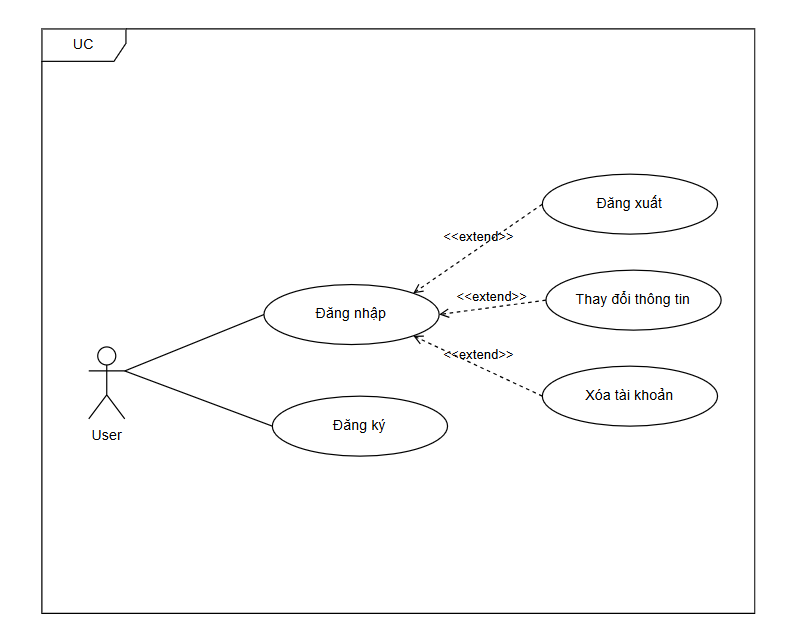
\includegraphics[width=0.8\textwidth]{Hinhve/Usecase_xac_thuc.png}
  \caption{Biểu đồ usecase Xác thực}
  \label{fig:use_case_xac_thuc}
\end{figure}
Usecase Xác thực bao gồm những chức năng chính sau (i) đăng nhập: người dùng nhập số điện thoại và mật khẩu để đăng nhập vào hệ thống, (ii) đăng ký: người dùng nhập các thông tin bắt buộc để đăng ký, (iii) đăng xuất: Đăng xuất khỏi tài khoản đang được đăng nhập.

\subsection{Biểu đồ use case phân rã Xác thực}
\label{subsection:2.2.3}
\begin{figure}[H]
  \centering
  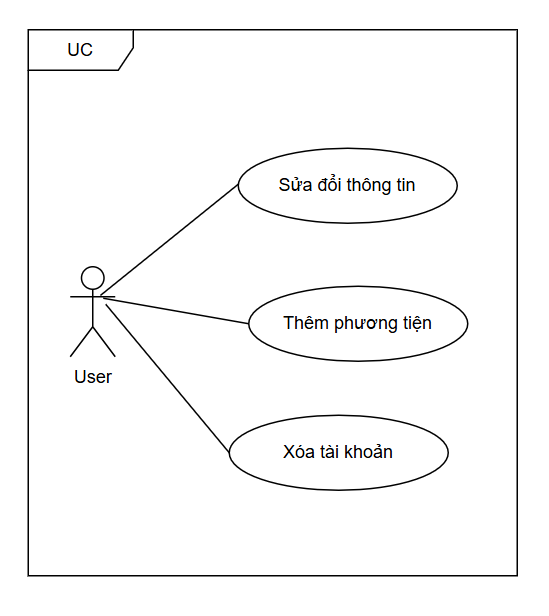
\includegraphics[width=0.8\textwidth]{Hinhve/Usecase_quan_ly_tai_khoan.png}
  \caption{Biểu đồ usecase Quản lý tài khoản}
  \label{fig:use_case_quan_ly_tai_khoan}
\end{figure}
Usecase Quản lý tài khoản bao gồm những chức năng chính sau (i) sửa đổi thông tin cá nhân: người dùng sửa đổi các thông tin cá nhân của mình, (ii) thêm phương tiện: người dùng thêm phương tiện muốn lái hộ, (iii) xóa tài khoản: người dùng xóa tài khoản của mình.

\subsection{Biểu đồ use case phân rã Đặt tài xế}
\label{subsection:2.2.4}
\begin{figure}[H]
  \centering
  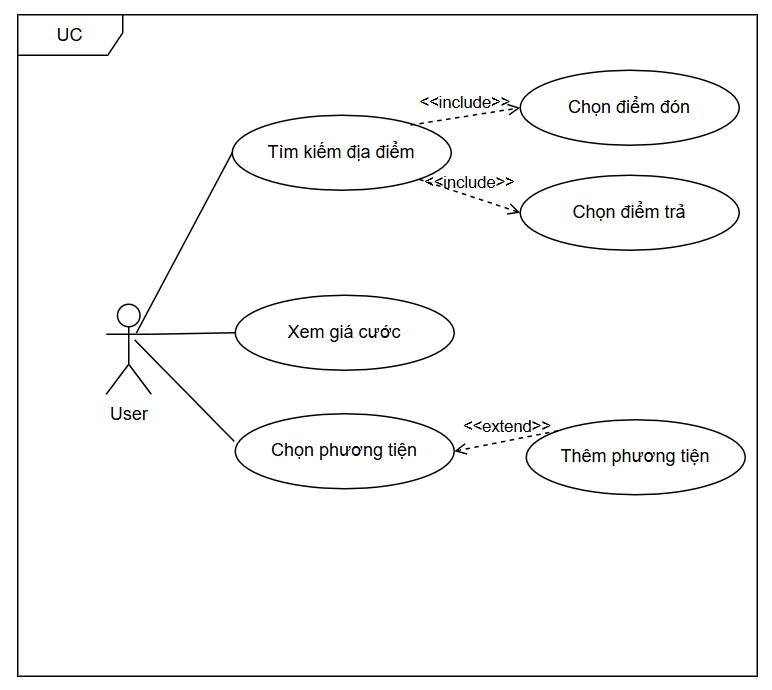
\includegraphics[width=0.8\textwidth]{Hinhve/Usecase_dat_tai_xe.png}
  \caption{Biểu đồ usecase Đặt tài xế}
  \label{fig:use_case_dat_tai_xe}
\end{figure}
Usecase Đặt tài xế bao gồm những chức năng chính sau (i) tìm kiếm địa điểm: người dùng nhập điểm đến, điểm đón, (ii) xem giá cước: người dùng xem giá cước của các chuyến đi, (iii) chọn phương tiện: người dùng chọn phương tiện để đặt chuyến.

\subsection{Biểu đồ use case phân rã Nhận chuyến}
\label{subsection:2.2.5}
\begin{figure}[H]
  \centering
  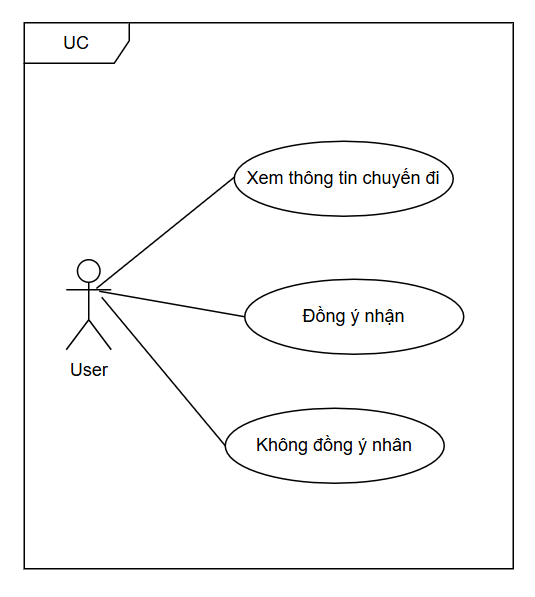
\includegraphics[width=0.8\textwidth]{Hinhve/Usecase_nhan_chuyen.png}
  \caption{Biểu đồ usecase Nhận chuyến}
  \label{fig:use_case_nhan_chuyen}
\end{figure}
Usecase Nhận chuyến bao gồm những chức năng chính sau (i) xem thông tin về chuyến đi: tài xế xem thông tin về chuyến đi như giá cước, địa điểm, (ii) đồng ý nhận: tài xế chấp nhận chuyến xe này, (iii) không đồng ý nhận: tài xế không chấp nhận chuyến đi và bỏ qua chuyến đi.


\subsection{Quy trình nghiệp vụ}
\label{section:2.3}
\subsection{Quy trình nghiệp vụ Tìm kiếm tài xế}
\label{subsection:2.3.1}
\begin{figure}[H]
  \centering
  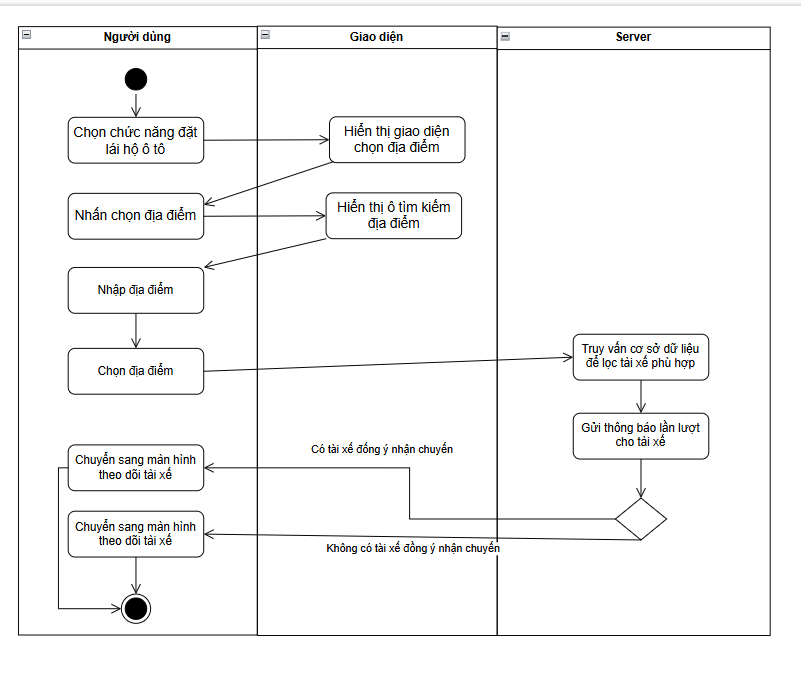
\includegraphics[width=0.8\textwidth]{Hinhve/quy_trinh_nghiep_vu_tim_kiem_tai_xe.png}
  \caption{Quy trình nghiệp vụ Tìm kiếm tài xế}
  \label{fig:quy_trinh_nghiep_vu_tim_kiem_tai_xe}
\end{figure}
Quy trình ở hình \ref{fig:quy_trinh_nghiep_vu_tim_kiem_tai_xe} mô tả nghiệp vụ tìm kiếm tài xế.
Người dùng có nhu cầu đặt lái hộ sẽ nhấn vào nút "Ô tô" trong phần "Dịch vụ lái xe hộ"
ở màn hình chính. Hệ thống sẽ hiển thị giao diện chọn vị trí để người
dùng chọn và nhập vị trí. Khi nhập vị trí, hệ thống sẽ hiển thị gợi ý vị
trí mà người dùng muốn đến.Sau khi người dùng chọn vị trí xong thì sẽ nhấn vào nút "Tiếp tục" để gửi 
dữ liệu tới server để thực hiện tính toán và trả về cho người dùng.


\section{Đặc tả chức năng}
\label{section:2.4}
\subsection{Đặc tả Đặt tài xế}
\label{subsection:2.4.1}

\renewcommand{\arraystretch}{1.5}
\begin{table}[H]
\centering
\begin{tabular}{|l|l|} 
\hline
\textbf{Mã usecase}             & UC-1                                                             \\ \hline
\textbf{Tên usecase}            & Đặt tài xế                                                       \\ \hline
\textbf{Mô tả}                  & Usecase này mô tả quá trình đặt tài xế của người dùng            \\ \hline
\textbf{Tác nhân}               & Người dùng                                                       \\ \hline
\textbf{Tiền điều kiện}         & Người dùng đăng nhập vào hệ thống                                \\ \hline
\textbf{Luồng sự kiện chính} & 
  \begin{tabular}[c]{@{}l@{}}1. Người dùng từ màn hình chính nhấn vào nút "Ô tô" của phần đặt xe hộ\\ 2. Người dùng tìm kiếm địa điểm đón và địa điểm trả\\ 3. Người dùng nhấn nút "Tiếp tục"\\ 4. Server tính toán quãng đường và giá tiền\\ 5. Người dùng xem quãng đường đi chuyển và giá tiền\\ 6. Người chọn phương tiện cần lái hộ\\ 7. Người dùng nhấn nút "Đặt tài xế"\\ 8. Server tìm kiếm tài xế phù hợp\end{tabular} \\ \hline
\textbf{Luồng sự kiện thay thế} & 8a. Hệ thống thông báo cho người dùng biết không tìm được tài xế \\ \hline
\textbf{Hậu điều kiện}          & Hệ thống chuyển sang màn hình theo dõi tài xế di chuyển          \\ \hline
\textbf{Luồng ngoại lệ}         & Không                     \\ \hline
\end{tabular}
\caption{Đặc tả usecase Đặt tài xế.}
\label{table:dac_ta_dat_tai_xe}
\end{table}
  
\subsection{Đặc tả use case Nhận chuyến}
\label{subsection:2.4.2}
\begin{table}[H]
\centering
\begin{tabular}{|l|l|}
\hline
\textbf{Mã usecase}    & UC-2                                               \\ \hline
\textbf{Tên usecase}   & Nhận chuyến                                        \\ \hline
\textbf{Mô tả}         & Usecase này mô tả quá trình nhận chuyến của tài xế \\ \hline
\textbf{Tác nhân}      & Tài xế                                             \\ \hline
\textbf{Tiền điều kiện} &
  \begin{tabular}[c]{@{}l@{}}- Người dùng đăng nhập vào hệ thống\\  - Người dùng ở chế độ online\end{tabular} \\ \hline
\textbf{Luồng sự kiện chính} &
  \begin{tabular}[c]{@{}l@{}}1. Hệ thống gửi thông báo tới tài xế đang có người muốn đặt chuyến\\ 2. Tài xế nhận thông báo về thông tin chuyến đi\\ 3. Người dùng nhấn nút "Tiếp tục"\end{tabular} \\ \hline
\textbf{Luồng sự kiện thay thế} &
  \begin{tabular}[c]{@{}l@{}}3a. Người dùng ấn nút 'X' để không chấp nhận chuyến xe\\ 3b. Hệ thống chờ 10 giây nếu người dùng không thực hiện thao \\ tác thì tự động bỏ qua chuyến xe.\end{tabular} \\ \hline
\textbf{Hậu điều kiện} & Hệ thống chuyển sang màn hình chuyến đi    \\ \hline
\textbf{Luồng ngoại lệ} & Không                                                            \\ \hline
\end{tabular}
\caption{Đặc tả usecase Nhận chuyến.}
\label{table:dac_ta_nhan_chuyen}
\end{table}

\subsection{Đặc tả use case Tìm kiếm tài xế}
\label{subsection:2.4.3}
\begin{table}[H]
\centering
\begin{tabular}{|l|l|}
\hline
\textbf{Mã usecase}             & UC-3                                                                                                    \\ \hline
\textbf{Tên usecase}            & Tìm kiếm tài xế                                                                                         \\ \hline
\textbf{Mô tả}                  & Usecase này mô tả quá trình tìm kiếm tài xế phù hợp                                                     \\ \hline
\textbf{Tác nhân}               & Người dùng, Hệ thống, Tài xế                                                                            \\ \hline
\textbf{Tiền điều kiện}         & \begin{tabular}[c]{@{}l@{}}- Người dùng đăng nhập vào hệ thống\\  - Tài xế ở chế độ online\end{tabular} \\ \hline
\textbf{Luồng sự kiện chính} &
  \begin{tabular}[c]{@{}l@{}}1. Người dùng gửi thông tin về chuyến đi đến server\\ 2. Server lọc ra những người phù hợp\\ 3. Server sắp xếp danh sách những người phù hợp\\ 4. Server gửi thông báo lần lượt tới danh sách tài xế\end{tabular} \\ \hline
\textbf{Luồng sự kiện thay thế} & Không                                                                                                   \\ \hline
\textbf{Hậu điều kiện}          & \begin{tabular}[c]{@{}l@{}}Server gửi thông báo cho người dùng đã tìm được tài xế\end{tabular}        \\ \hline
\textbf{Luồng ngoại lệ}         & Hệ thống gửi thông báo không tìm được tài xế                                                            \\ \hline
\end{tabular}
\caption{Đặc tả usecase Tìm kiếm tài xế.}
\label{table:dac_ta_tim_kiem_tai_xe}
\end{table}

\subsection{Đặc tả use case Chỉnh sửa thông tin}
\label{subsection:2.4.4}
\begin{table}[H]
\centering
\begin{tabular}{|l|l|}
\hline
\textbf{Mã usecase}             & UC-4                                                                                             \\ \hline
\textbf{Tên usecase}            & Thay đổi thông tin cá nhân                                                                       \\ \hline
\textbf{Mô tả}                  & \begin{tabular}[c]{@{}l@{}}Usecase này mô tả quá trình thay đổi thông tin cá nhân\end{tabular} \\ \hline
\textbf{Tác nhân}               & Người dùng                                                                                       \\ \hline
\textbf{Tiền điều kiện}         & - Người dùng đăng nhập vào hệ thống                                                              \\ \hline
\textbf{Luồng sự kiện chính} &
  \begin{tabular}[c]{@{}l@{}}1. Người dùng nhấn nút "Tài khoản"\\ 2. Hệ thống hiển thị thông tin của người dùng\\ 3. Người dùng nhập thông tin cần thay đổi\\ 4. Người dùng nhấn nút "Cập nhật"\end{tabular} \\ \hline
\textbf{Luồng sự kiện thay thế} & 4a. Hệ thống thông báo cập nhật thành                                                            \\ \hline
\textbf{Hậu điều kiện}          & Hệ thống hiển thị thông tin mới được chỉnh sửa                                                   \\ \hline
\textbf{Luồng ngoại lệ}         & \begin{tabular}[c]{@{}l@{}}Hệ thống gửi thông báo chỉnh sửa thông tin thất\\ bại\end{tabular}    \\ \hline
\end{tabular}
\caption{Đặc tả usecase Thay đổi thông tin cá nhân.}
\label{table:dac_ta_thay_doi_thong_tin_ca_nhan}
\end{table}

\section{Yêu cầu phi chức năng}
\label{section:2.5}
Trong phần này, sinh viên đưa ra các yêu cầu khác nếu có, bao gồm các yêu cầu phi chức năng như hiệu năng, độ tin cậy, tính dễ dùng, tính dễ bảo trì, hoặc các yêu cầu về mặt kỹ thuật như về CSDL, công nghệ sử dụng, v.v.


\end{document}